\documentclass[11pt,a4paper]{article}
\usepackage[T1]{fontenc}
\usepackage[utf8]{inputenc}
\usepackage{lmodern}
\usepackage[margin=2.5cm]{geometry}
\usepackage{booktabs,graphicx,amsmath,amssymb,enumitem,xcolor,array}
\usepackage[numbers,sort&compress]{natbib}
\usepackage[hidelinks]{hyperref}
\newcommand{\NRec}{120}
\newcommand{\NPart}{24}
\newcommand{\NEvMin}{12}
\newcommand{\NEvMed}{46}
\newcommand{\NEvMax}{216}
\newcommand{\AccFaith}{95.8}
\newcommand{\FFaith}{0.108}
\newcommand{\FFaithLo}{0.089}
\newcommand{\FFaithHi}{0.128}
\newcommand{\SFaith}{0.32}
\newcommand{\RemFaith}{0.267}
\newcommand{\ValFaith}{0.058}
\newcommand{\ShiftFaith}{0.000}
\newcommand{\AccPos}{95.8}
\newcommand{\FPos}{0.025}
\newcommand{\FPosLo}{0.011}
\newcommand{\FPosHi}{0.039}
\newcommand{\SPos}{0.19}
\newcommand{\RemPos}{0.067}
\newcommand{\ValPos}{0.008}
\newcommand{\ShiftPos}{0.000}
\newcommand{\AccRand}{95.8}
\newcommand{\FRand}{-0.011}
\newcommand{\FRandLo}{-0.028}
\newcommand{\FRandHi}{0.006}
\newcommand{\SRand}{0.19}
\newcommand{\RemRand}{-0.008}
\newcommand{\ValRand}{-0.025}
\newcommand{\ShiftRand}{0.000}

\newcommand{\NLlmConfigs}{9}
\newcommand{\MaxLevel}{0}
\newcommand{\AccMaxLo}{0.59}
\newcommand{\SpearmanAccF}{0.53}
\newcommand{\DeepEnrAcc}{52.5}
\newcommand{\DeepEnrF}{0.097}
\newcommand{\DeepEnrFLo}{0.072}
\newcommand{\DeepEnrFHi}{0.122}
\newcommand{\DeepEnrNoise}{0.02}
\newcommand{\DeepEnrS}{0.96}
\newcommand{\DeepPlAcc}{49.2}
\newcommand{\DeepPlF}{0.139}
\newcommand{\DeepPlFLo}{0.083}
\newcommand{\DeepPlFHi}{0.200}
\newcommand{\DeepPlNoise}{0.17}
\newcommand{\DeepPlS}{0.56}
\newcommand{\LunaEnrAcc}{65.0}
\newcommand{\LunaEnrF}{0.169}
\newcommand{\LunaEnrFLo}{0.122}
\newcommand{\LunaEnrFHi}{0.217}
\newcommand{\LunaEnrNoise}{0.11}
\newcommand{\LunaEnrS}{0.90}
\newcommand{\LunaPlAcc}{35.0}
\newcommand{\LunaPlF}{0.047}
\newcommand{\LunaPlFLo}{-0.033}
\newcommand{\LunaPlFHi}{0.131}
\newcommand{\LunaPlNoise}{0.39}
\newcommand{\LunaPlS}{0.33}

\newcommand{\HDeepPlAcc}{57.5}
\newcommand{\HDeepPlF}{0.101}
\newcommand{\HDeepPlFLo}{0.063}
\newcommand{\HDeepPlFHi}{0.142}
\newcommand{\HLunaPlAcc}{59.6}
\newcommand{\HLunaPlF}{0.062}
\newcommand{\HLunaPlFLo}{0.032}
\newcommand{\HLunaPlFHi}{0.094}
\newcommand{\HomeRefAcc}{59.2}
\newcommand{\HomeRefAccLo}{52.3}
\newcommand{\HomeRefAccHi}{66.3}
\newcommand{\HomeAllAcc}{60.0}
\newcommand{\HomeRefF}{0.182}
\newcommand{\HomeMaxAccLo}{0.53}
\newcommand{\XAFaithfulGap}{0.170}
\newcommand{\XAFaithfulGapLo}{0.148}
\newcommand{\XAFaithfulGapHi}{0.192}
\newcommand{\XAFaithfulPrec}{1.00}
\newcommand{\XAFaithfulChance}{0.26}
\newcommand{\XAPositionalGap}{0.044}
\newcommand{\XAPositionalGapLo}{0.029}
\newcommand{\XAPositionalGapHi}{0.057}
\newcommand{\XAPositionalPrec}{0.19}
\newcommand{\XAPositionalChance}{0.26}
\newcommand{\XARandomGap}{0.001}
\newcommand{\XARandomGapLo}{-0.010}
\newcommand{\XARandomGapHi}{0.013}
\newcommand{\XARandomPrec}{0.24}
\newcommand{\XARandomChance}{0.26}
\newcommand{\XALunaPlGap}{0.038}
\newcommand{\XALunaPlGapLo}{0.020}
\newcommand{\XALunaPlGapHi}{0.057}
\newcommand{\XALunaPlPrec}{0.39}
\newcommand{\XALunaPlChance}{0.25}
\newcommand{\XADeepEnrGap}{0.081}
\newcommand{\XADeepEnrGapLo}{0.061}
\newcommand{\XADeepEnrGapHi}{0.101}
\newcommand{\XADeepEnrPrec}{0.38}
\newcommand{\XADeepEnrChance}{0.25}
\newcommand{\XALunaEnrGap}{0.050}
\newcommand{\XALunaEnrGapLo}{0.036}
\newcommand{\XALunaEnrGapHi}{0.063}
\newcommand{\XALunaEnrPrec}{0.29}
\newcommand{\XALunaEnrChance}{0.22}
\newcommand{\XADeepPlGap}{0.080}
\newcommand{\XADeepPlGapLo}{0.060}
\newcommand{\XADeepPlGapHi}{0.100}
\newcommand{\XADeepPlPrec}{0.46}
\newcommand{\XADeepPlChance}{0.25}
\newcommand{\XHFaithfulGap}{0.142}
\newcommand{\XHFaithfulGapLo}{0.120}
\newcommand{\XHFaithfulGapHi}{0.164}
\newcommand{\XHFaithfulPrec}{1.00}
\newcommand{\XHFaithfulChance}{0.48}
\newcommand{\XHPositionalGap}{0.027}
\newcommand{\XHPositionalGapLo}{0.019}
\newcommand{\XHPositionalGapHi}{0.035}
\newcommand{\XHPositionalPrec}{0.60}
\newcommand{\XHPositionalChance}{0.48}
\newcommand{\XHRandomGap}{0.024}
\newcommand{\XHRandomGapLo}{0.016}
\newcommand{\XHRandomGapHi}{0.033}
\newcommand{\XHRandomPrec}{0.47}
\newcommand{\XHRandomChance}{0.48}
\newcommand{\XHDeepPlGap}{0.046}
\newcommand{\XHDeepPlGapLo}{0.029}
\newcommand{\XHDeepPlGapHi}{0.064}
\newcommand{\XHDeepPlPrec}{0.42}
\newcommand{\XHDeepPlChance}{0.40}
\newcommand{\XHLunaPlGap}{0.055}
\newcommand{\XHLunaPlGapLo}{0.039}
\newcommand{\XHLunaPlGapHi}{0.071}
\newcommand{\XHLunaPlPrec}{0.45}
\newcommand{\XHLunaPlChance}{0.42}
\newcommand{\XHLunaEnrGap}{0.066}
\newcommand{\XHLunaEnrGapLo}{0.050}
\newcommand{\XHLunaEnrGapHi}{0.083}
\newcommand{\XHLunaEnrPrec}{0.52}
\newcommand{\XHLunaEnrChance}{0.44}
\newcommand{\XHDeepEnrGap}{0.048}
\newcommand{\XHDeepEnrGapLo}{0.029}
\newcommand{\XHDeepEnrGapHi}{0.067}
\newcommand{\XHDeepEnrPrec}{0.38}
\newcommand{\XHDeepEnrChance}{0.38}
\newcommand{\DecAccAdl}{95.8}
\newcommand{\DecAccAdlLo}{92.5}


% Marks text that depends on experiments that have not been run yet.
\newcommand{\pending}[1]{\par\medskip\noindent\fbox{\parbox{0.94\linewidth}{\small\textbf{Pending.} #1}}\medskip}

\title{When Can an Activity-Recognition Agent Be Trusted to Act?\\
Counterfactual Faithfulness of LLM Explanations and\\
Accountability in Ambient Assisted Living}
\author{Quang-Vinh Dang\\
\small British University Vietnam, Hung Yen, Vietnam\\
\small \texttt{vinh.dq4@buv.edu.vn} \quad ORCID 0000-0002-3877-8024}
\date{}

\begin{document}
\maketitle

\begin{abstract}
Large language models (LLMs) are increasingly placed on top of activity recognition systems in smart homes and ambient assisted living (AAL). They label activities, explain their conclusions, and may trigger actions such as alerting a caregiver or requesting emergency assistance. Their explanations are fluent, but fluent explanations can describe correlations that the model never used, so explanation quality becomes a safety question as well as an interpretability one. This chapter asks when such an agent can justifiably be allowed to act. We propose a counterfactual faithfulness protocol: for every explanation that cites sensor events as evidence, we intervene on the cited events (removal, value change, temporal shift) and on a size-matched set of uncited events, and test whether the agent's conclusion moves with the cited evidence and not with the rest. We validate the protocol on CASAS scripted-ADL data using three agents that share one classifier, and so one accuracy, but cite evidence by different rules; the protocol separates them. We then apply it to nine configurations of six language models under plain and context-enriched prompting. On scripted activities no configuration was accurate enough to be allowed to do more than log, and accuracy and faithfulness were only loosely related. On free-living data from 77 homes, where sensor names carry meaning, zero-shot models matched a trained classifier, so recognition alone is not the obstacle. The explanations are: when a classifier decides and a language model only points at the supporting events, the cited events track the classifier's evidence only modestly better than chance on scripted data and barely above chance on free-living data. We relate measured faithfulness to accountability under the GDPR, the EU AI Act and the Vietnamese regulatory setting, covering the evidentiary weight of a model-generated inference, the consent of monitored older adults, and the allocation of responsibility among developers, deployers and caregivers. We close with a graduated authority ladder that ties measured evidence to permitted actions, from logging to caregiver notification to irreversible actions that always require human confirmation, and show that with the decision system held fixed the ladder assigns different levels to different explainers. Sensitivity to input changes is necessary but not sufficient evidence of sound reasoning, and we say what the protocol cannot show.
\end{abstract}

\section{Introduction: from activity recognition to agents that explain and act}

Activity recognition in the home began as classification: a window of motion, door and item-use events goes in, a label comes out \cite{cook2013casas}. A label is passive. Someone reads it, or nobody does, and the cost of a wrong label is a wrong dashboard entry.

Language models change the role of the recogniser in two ways. First, they are being used as reasoning layers over sensor data, sometimes with no task-specific training, and they can report on a day of sensor events in plain prose \cite{ji2024hargpt,civitarese2024zeroshot}. Second, they are wrapped in agent frameworks that can call tools: send a message, place a call, change a device state. Once the output of the model can cause something to happen to a frail person living alone, the properties we need from it change. Accuracy on a benchmark is no longer enough, because the person who has to decide whether to act on the output, or to trust that the system acted correctly, relies on the explanation that comes with it.

That explanation is the weak point. Language models produce explanations that read well, and several studies show that what they say about their own reasoning need not match what drove their answer. Biasing features in the input change the answer without being mentioned, and stated chain-of-thought steps can be unrelated to the outcome \cite{turpin2023say,lanham2023faithfulness}. Faithfulness, in the sense of an explanation that reflects the process that produced the decision, is a long-standing concern in interpretable NLP \cite{jain2019attention,jacovi2020faithfully}. In a monitoring setting an unfaithful explanation does particular damage. A caregiver who sees ``motion in the kitchen at 03:12, then no motion in the bedroom, so the resident has probably fallen'' will reasonably check the kitchen, whether or not the model's decision depended on those events. If the story was invented after the fact, the caregiver's check is aimed at the wrong evidence, and neither the caregiver nor an auditor can tell.

The question of this chapter follows directly: \emph{when can an activity-recognition agent be trusted to act?} The answer is not ``never'', and it is not ``when it is accurate''. Authority has to be earned in steps and the evidence for it has to be measured, for the decision and for the explanation separately. We answer in two parts. The first is empirical and operational. Section~\ref{sec:protocol} defines a counterfactual faithfulness protocol that can be run on any agent that reads a sensor log and cites events. Section~\ref{sec:pilot} validates it on public data. The second part is normative. Section~\ref{sec:accountability} asks what a measured faithfulness score is worth as evidence in the legal frameworks that govern AAL in the European Union and Vietnam, and Section~\ref{sec:ladder} turns the answer into a graduated authority ladder. Section~\ref{sec:limits} states the limits. The code, data pointers and results are in the accompanying repository.

\paragraph{Contributions.}
(i) A protocol that scores explanation faithfulness by intervention on the cited events, against a size-matched control on uncited events, with a null control for the agent's own instability. (ii) A validity check showing that the protocol separates agents of identical accuracy. (iii) An analysis connecting the score to the evidentiary, consent and responsibility questions raised by AAL deployments. (iv) An authority ladder that gives the score a decision role without making it the only gate. (v) Two further experiments: free-living data, where language models are competitive, and an explain-only setting in which a classifier decides and the language model only explains, which isolates the explanation as the weak component.

\section{Background}
\label{sec:background}

\subsection{LLM reasoning over ambient and wearable sensing}
Ambient activity recognition has used hand-crafted features with classical classifiers, then deep sequence models, on datasets such as those from the CASAS testbeds \cite{cook2013casas}. Recent work asks whether general-purpose language models can recognise activities from raw or lightly processed sensor streams with little or no training: HARGPT prompts a model with raw inertial data \cite{ji2024hargpt}, and Civitarese et al.\ evaluate zero-shot recognition of activities of daily living from ambient sensor events, including the use of context such as sensor placement and activity definitions \cite{civitarese2024zeroshot}. The common finding is that language models can be competitive on coarse activities when given context, and that results are sensitive to how the sensor data is described. Our study follows the same setting, because it is where agents are being built, but its target is not accuracy.

\subsection{Failure modes of generated explanations}
Three failure modes matter for monitoring. \emph{Confabulation}: the explanation names evidence that the decision did not depend on. \emph{Omission}: the decision depends on something the explanation does not mention, such as a prior about the time of day. \emph{Fabrication}: the explanation cites events that are not in the log. The first two are about faithfulness and can be probed only by intervening on the input; reading the explanation cannot reveal them. The third can be checked directly, and our harness records it as an invalid citation.

\subsection{Measuring faithfulness by intervention}
In text classification, faithfulness is often measured by removing the rationale a model gives and checking how much its confidence falls (\emph{comprehensiveness}), and by keeping only the rationale and checking how much confidence survives (\emph{sufficiency}) \cite{deyoung2020eraser}. Our protocol borrows both ideas and adapts them to sensor logs, where an ``input token'' is a timestamped event with a sensor identity and a reading, and where evidence can be altered in ways that have no text analogue: the reading can change and the event can move in time. Two further additions matter in practice. We compare with a matched control on uncited events, because removing any ten events from a short log can change a conclusion, and a null control, because an agent that flips its answer when nothing relevant changed has a noise floor that must be subtracted from any claim of sensitivity.

\section{A counterfactual faithfulness protocol for sensor-grounded explanations}
\label{sec:protocol}

\subsection{Setting}
A \emph{recording} is a time-ordered log $L=(e_1,\dots,e_n)$ of events $e_i=(t_i,s_i,v_i)$, with timestamp, sensor identity and reading. An \emph{agent} maps a log to a triple $(y, C, x)$: a conclusion $y$ from a closed label set, a cited set $C\subseteq\{1,\dots,n\}$ of at most $k$ event indices, and a free-text explanation $x$. We use $k=10$. The protocol uses $y$ and $C$; the text $x$ is retained for audit. A citation outside $\{1,\dots,n\}$ is counted as invalid and dropped.

\subsection{Interventions}
Let $\pi$ be an operation on a log and a set of positions. We use three families, chosen to cover what an explanation might claim about an event.
\begin{description}[leftmargin=1.2cm,style=nextline]
\item[Removal.] $\pi_{\mathrm{rem}}(L,A)$ deletes the events at positions $A$. This tests whether the event is needed.
\item[Value change.] $\pi_{\mathrm{val}}(L,A)$ replaces each reading by its inverse (ON$\leftrightarrow$OFF, PRESENT$\leftrightarrow$ABSENT, OPEN$\leftrightarrow$CLOSE, START$\leftrightarrow$END) and sets an analogue level, such as water flow or burner level, to zero. Events with no defined inverse are left unchanged. This tests whether the content of the reading matters, not only its existence.
\item[Temporal shift.] $\pi_{\mathrm{shift}}(L,A)$ moves the events at $A$ later by a fixed offset and re-sorts the log. This tests whether the order and timing that the explanation relies on actually matter.
\end{description}
For each family $f$ we form two logs from the same base: $\pi_f(L,C)$ on the cited events, and $\pi_f(L,U)$ where $U$ is a uniformly random subset of the uncited events with $|U|=|C|$. The matched size keeps the amount of change equal, so a difference between the two can be attributed to \emph{which} events were touched.

\subsection{Scores}
Let $y_0$ be the conclusion on the base log and $y_f^{C}$, $y_f^{U}$ the conclusions after intervening on cited and uncited events. The \emph{conclusion-change indicator} is $\delta(y,y')=\mathbb 1[y\neq y']$. The per-family faithfulness gap and the overall score are
\begin{equation}
\Delta_f=\delta(y_0,y_f^{C})-\delta(y_0,y_f^{U}),\qquad F=\frac13\sum_{f\in\{\mathrm{rem},\mathrm{val},\mathrm{shift}\}}\Delta_f,
\end{equation}
averaged over recordings with a well-formed answer and at least one valid citation. $F\in[-1,1]$. An explanation is faithful to the degree that $F$ is positive: interventions on cited evidence move the conclusion, interventions on uncited evidence do not. Two companion quantities complete the report.
\begin{itemize}[nosep]
\item \textbf{Sufficiency} $S=\Pr[\,y(\pi_{\mathrm{keep}}(L,C))=y_0\,]$, where $\pi_{\mathrm{keep}}$ keeps only the cited events: does the cited evidence alone carry the conclusion?
\item \textbf{Noise floor} $N=\Pr[\,y(L;\eta)\neq y_0\,]$, where $\eta$ is a content-free change to the request (we add an inert request identifier): how often does the agent contradict itself when nothing relevant changed?
\end{itemize}
Intervals are percentile bootstrap intervals over participants, not recordings, because recordings from one person are not independent.

\subsection{What a score does and does not say}
$F$ is the \emph{necessity} side of faithfulness, measured at the level of conclusions. It will be small for agents whose evidence is redundant, because deleting the ten most important of forty supporting events may leave enough to reach the same conclusion. $F$ therefore has no absolute scale, and Section~\ref{sec:pilot} calibrates it against a reference agent that is faithful by construction on the same data. It is also sensitive to the choice of interventions: a bag-of-events classifier is blind to temporal shift, so $\Delta_{\mathrm{shift}}=0$ for it, correctly. The score tests whether the cited evidence is \emph{used}; it does not test whether the use is \emph{sound}. We return to this in Section~\ref{sec:limits}.

\section{Pilot study on CASAS: accuracy versus faithfulness}
\label{sec:pilot}

\subsection{Data}
We use the CASAS scripted-ADL recordings without errors, released under CC~BY~4.0 \cite{casas_zenodo_adl}. Participants perform five tasks in a smart apartment: making a phone call, washing hands, cooking oatmeal, eating (with a medicine container), and cleaning the dishes. There are \NRec{} recordings from \NPart{} participants, each between \NEvMin{} and \NEvMax{} events (median \NEvMed). The sensors are PIR motion sensors, item-use sensors for eight objects, a cabinet door sensor, analogue water-flow and burner sensors, and the telephone. The task number is the label. The scripted setting is cleaner than free living, so the accuracy numbers below are an upper bound on what an agent would reach at home. We chose it for a different reason: the activity labels, the sensor semantics and the layout are documented, which allows a controlled comparison of plain and context-enriched prompting.

\subsection{Validating the protocol with reference agents}
\label{sec:reference}
Before using the protocol to judge language models we ask whether it can tell a faithful explanation from an unfaithful one when we know the answer. We train one multinomial logistic-regression classifier on log-counts of (sensor, reading) tokens, with leave-one-participant-out evaluation, and attach three citing rules to it.
\begin{itemize}[nosep]
\item \emph{Faithful:} cite the ten events whose tokens contribute most to the decision margin.
\item \emph{Positional:} cite the first ten events, a plausible story (``the activity began with\dots'') that is independent of the decision.
\item \emph{Random:} cite ten randomly chosen events.
\end{itemize}
All three share the same predictions, so their accuracy is identical, \AccFaith\% across \NRec{} recordings. Table~\ref{tab:ref} and Figure~\ref{fig:ref} give the protocol output.

\begin{table}[t]
\centering
\begin{tabular}{lcccc}
\toprule
Citing rule & Accuracy & $F$ [95\% CI] & $S$ & Noise floor \\
\midrule
Faithful (cites top contributions) & 95.8\% & 0.108 [0.089, 0.128] & 0.32 & 0.00 \\
Positional (cites first events) & 95.8\% & 0.025 [0.011, 0.039] & 0.19 & 0.00 \\
Random (cites random events) & 95.8\% & -0.011 [-0.028, 0.006] & 0.19 & 0.00 \\
\bottomrule
\end{tabular}

\caption{Protocol output for three agents with the same classifier and the same accuracy. $F$: faithfulness score; $S$: sufficiency; noise floor: flip rate under a content-free change of the request. Intervals are participant-level bootstrap intervals.}
\label{tab:ref}
\end{table}

\begin{figure}[t]
\centering
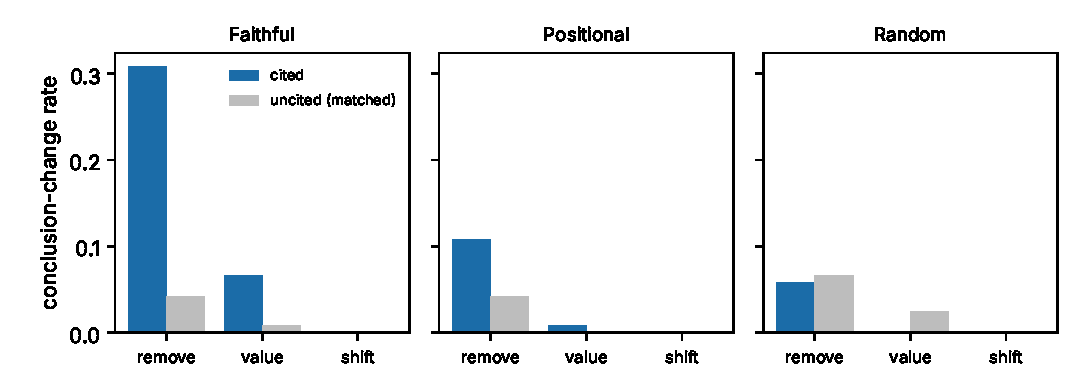
\includegraphics[width=\linewidth]{figures/reference_flip_rates.pdf}
\caption{Conclusion-change rates after intervening on cited events and on a size-matched set of uncited events, by intervention family and citing rule. The faithful agent's removal gap is \RemFaith; the temporal-shift bars are empty because a bag-of-events classifier ignores order.}
\label{fig:ref}
\end{figure}

Three observations. First, accuracy does not predict faithfulness: the three agents are indistinguishable by accuracy and ordered by $F$, \FFaith{} for the faithful rule (95\% CI \FFaithLo{} to \FFaithHi) against \FRand{} for random citation (interval \FRandLo{} to \FRandHi, which contains zero, as it should). Second, the positional rule scores \FPos{} (\FPosLo{} to \FPosHi{}), slightly above zero. That is not a defect of the metric: the first events of a recording are informative in this scripted data, so a story that is independent of the decision by construction still touches some evidence the decision uses. Third, absolute values are low. Even the faithful agent has $F=\FFaith$, because the classifier has many redundant features and the removal gap is \RemFaith{} while the value-change gap is \ValFaith. The score is useful for ordering agents on the same data and for comparison with a calibrated reference; it should not be read as a percentage of faithfulness. The noise floor is zero here because the reference agents are deterministic.

\subsection{Language-model agents under plain and context-enriched prompting}
\label{sec:llm}
\paragraph{Design.} Models are queried at temperature zero, with optional reasoning modes switched off where the interface allows it, and answer in the JSON format above. The \emph{plain} prompt gives the raw log (relative time, sensor identifier, reading), the five labels and the output format. The \emph{context-enriched} prompt adds the sensor dictionary (item-use sensors named, analogue sensors explained, rooms identified) and a one-line definition of each activity. Each recording yields one base query, one null query, one sufficiency query and six intervention queries, nine queries per recording per configuration. The study was run with whatever access was available, which determined its size. Two models, GPT-6-Luna (proprietary) and DeepSeek-V4.1-Flash (open weights), were run on all \NRec{} recordings under both prompts. Three further models were run on smaller subsets chosen to be balanced over the five activities and spread over participants, because of free-tier rate limits: Laguna-S-2.1 (20 recordings, both prompts) and gpt-oss-120b, gpt-oss-20b and Qwen3.8-27B (15 recordings, plain prompt only). Table~\ref{tab:llm} reports every configuration that returned answers for at least 15 recordings; the intervals for the 15- and 20-recording runs are wide and those rows should be read as indications only. Configurations that did not meet this bar are listed in Section~\ref{sec:limits}.

\begin{table}[t]
\centering
\footnotesize
\setlength{\tabcolsep}{4pt}
\begin{tabular}{llrccccc}
\toprule
Model & Prompt & $n$ & Accuracy [95\% CI] & $F$ [95\% CI] & $S$ & Noise & Level \\
\midrule
deepseek-v4.1-flash-1017 & enriched & 120 & 0.53 [0.48, 0.57] & 0.10 [0.07, 0.12] & 0.96 & 0.02 & 0 \\
deepseek-v4.1-flash-1017 & plain & 120 & 0.49 [0.46, 0.53] & 0.14 [0.08, 0.20] & 0.56 & 0.17 & 0 \\
gpt-6-luna & enriched & 120 & 0.65 [0.59, 0.72] & 0.17 [0.12, 0.22] & 0.90 & 0.11 & 0 \\
gpt-6-luna & plain & 120 & 0.35 [0.27, 0.42] & 0.05 [-0.03, 0.13] & 0.33 & 0.39 & 0 \\
laguna-s-2.1 (free) & enriched & 20 & 0.35 [0.15, 0.55] & 0.06 [0.00, 0.12] & 1.00 & 0.00 & 0 \\
laguna-s-2.1 (free) & plain & 20 & 0.45 [0.25, 0.65] & 0.12 [0.00, 0.25] & 0.60 & 0.15 & 0 \\
gpt-oss-120b & plain & 15 & 0.40 [0.20, 0.67] & 0.11 [-0.04, 0.27] & 0.40 & 0.53 & 0 \\
gpt-oss-20b & plain & 15 & 0.13 [0.00, 0.33] & 0.13 [-0.04, 0.29] & 0.60 & 0.40 & 0 \\
qwen3.8-27b & plain & 15 & 0.20 [0.00, 0.40] & 0.00 [0.00, 0.00] & 1.00 & 0.00 & 0 \\
\bottomrule
\end{tabular}

\caption{Language-model agents on CASAS scripted-ADL recordings. $n$: recordings with a well-formed answer; $F$: faithfulness score; $S$: sufficiency; Noise: flip rate under a content-free change of the request; Level: authority level from the ladder of Section~\ref{sec:ladder}. Intervals are participant-level bootstrap intervals. For comparison, the reference classifier reaches 95.8\% accuracy and the faithful reference agent $F=\FFaith$.}
\label{tab:llm}
\end{table}

\begin{figure}[t]
\centering
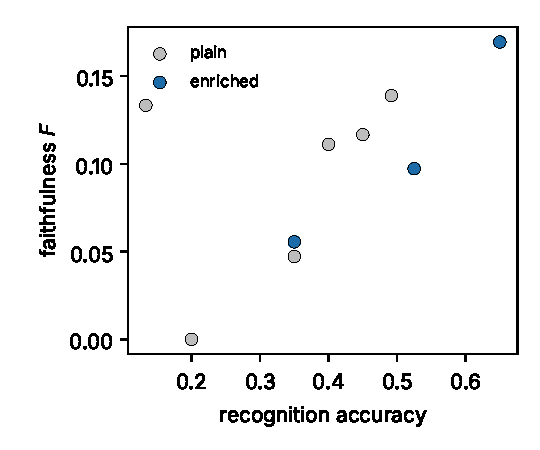
\includegraphics[width=0.6\linewidth]{figures/accuracy_vs_faithfulness.pdf}
\caption{Recognition accuracy against faithfulness score for the nine language-model configurations in Table~\ref{tab:llm}.}
\label{fig:acc-faith}
\end{figure}

\paragraph{Recognition is far below the reference classifier.} The best configuration, GPT-6-Luna with context, reaches \LunaEnrAcc\% accuracy against 95.8\% for the logistic-regression reference trained on the other participants. Errors are structured, not random. With context, DeepSeek never predicts \emph{clean} or \emph{eat}: 78 of its 120 answers are \emph{cook}, because all three activities take place around the same sensors. GPT-6-Luna with context is perfect on \emph{make\_phone\_call} and \emph{cook} (24 of 24 each), but sends 14 of 24 \emph{clean} recordings and 11 of 24 \emph{eat} recordings to \emph{cook}. Without context, GPT-6-Luna labels 17 of 24 phone calls as hand washing. The models run on the plain prompt only reached between 13\% and 45\% on their small subsets, and Qwen3.8-27B answered \emph{wash\_hands} for all 15 recordings.

\paragraph{Context changes accuracy, faithfulness and stability by different amounts.} For GPT-6-Luna, adding context raises accuracy from \LunaPlAcc\% to \LunaEnrAcc\%, the faithfulness score from \LunaPlF{} (95\% CI \LunaPlFLo{} to \LunaPlFHi) to \LunaEnrF{} (\LunaEnrFLo{} to \LunaEnrFHi), sufficiency from \LunaPlS{} to \LunaEnrS{}, and lowers the noise floor from \LunaPlNoise{} to \LunaEnrNoise. The plain-prompt noise floor is large: GPT-6-Luna changes its answer in about four of ten recordings when only an inert request identifier changes, which is more than the gap between its cited and uncited interventions. A faithfulness claim about that configuration would be unsafe without the matched control and the null control. For DeepSeek, context raises accuracy only slightly (\DeepPlAcc\% to \DeepEnrAcc\%, within the intervals) while sufficiency rises from \DeepPlS{} to \DeepEnrS{} and the noise floor falls from \DeepPlNoise{} to \DeepEnrNoise. Its faithfulness score nominally \emph{falls}, from \DeepPlF{} to \DeepEnrF, although the intervals overlap, so we do not claim a decrease. We read this as a model that settles on a stable, context-driven answer (mostly \emph{cook}) that depends less on any particular cited event.

\paragraph{Accuracy and faithfulness are only loosely related.} Across the nine configurations the rank correlation between accuracy and $F$ is \SpearmanAccF; with nine points that is descriptive, not a test. The configurations show why. gpt-oss-20b is correct on 13\% of recordings yet has $F=0.13$ (interval $-0.04$ to $0.29$), higher than GPT-6-Luna's without context (0.05) at 35\% accuracy. Qwen3.8-27B has $F=0$ exactly because its answer never changes: an agent that ignores its input is perfectly stable and perfectly unfaithful. Most striking, faithfulness is \emph{higher} on the recordings the agent gets wrong: for GPT-6-Luna with context $F$ is 0.132 on correct answers and 0.238 on wrong ones, and for DeepSeek with context 0.042 and 0.158. Conclusions that are fragile are both easier to flip and more often wrong, so a high score can reflect indecision as well as use of evidence.

\paragraph{Explanations can name things the log does not contain.} In the plain prompt the model is told nothing about what the sensor identifiers mean, yet explanations supply meanings. One gpt-oss-20b explanation for recording p01.t5 (clean, answered \emph{cook}) reports that the resident ``turned on the stove (M15), oven (M16) and microwave (M17)''. These are motion sensors, and the log contains no device of those names. The intervention protocol would not flag this, since the cited events exist and may even move the answer, which is why the text of explanations should be audited as well as perturbed.

\subsection{Free-living segments: where language models are competitive}
\label{sec:home}
The scripted recordings use opaque identifiers (M13, I05), so a language model has to be told what they mean. Real homes often use sensors named for what they sense. We therefore repeat the study on the CASAS labelled long-term data (82 homes, released under CC~BY~4.0 on Zenodo), where sensor names such as \texttt{KitchenAStove}, \texttt{BathroomASink} and \texttt{BedroomABed} carry meaning. From annotated activity episodes we keep those that do not overlap another annotation and contain between 10 and 80 events, merge variants (Cook\_Breakfast, Cook\_Dinner, \dots) and sample episodes for eight activities (sleep, personal hygiene, toilet, cook, eat, watch TV, work, wash dishes), at most three per home and activity. The explain-only experiment of Section~\ref{sec:explain} uses 600 segments (75 per activity) from 77 homes, median 24 events. The full protocol needs nine queries per segment, so for the language-model runs we use a balanced subset of 240 segments (30 per activity) from 70 homes, with the plain prompt only because of budget. An earlier pilot on 120 segments that also included the enriched prompt is kept in the repository. The comparison classifier is the same logistic regression, evaluated leave-one-home-out.

\begin{table}[t]
\centering
\footnotesize
\setlength{\tabcolsep}{4pt}
\begin{tabular}{llcccccc}
\toprule
Agent & Prompt & Accuracy [95\% CI] & $F$ [95\% CI] & $S$ & Noise & Level \\
\midrule
logistic regression & -- & 0.59 [0.52, 0.66] & -- & -- & -- & -- \\
deepseek-v4.1-flash & plain & 0.57 [0.51, 0.64] & 0.10 [0.06, 0.14] & 0.97 & 0.04 & 0 \\
gpt-6-luna & plain & 0.60 [0.53, 0.66] & 0.06 [0.03, 0.09] & 0.93 & 0.07 & 0 \\
\bottomrule
\end{tabular}

\caption{Free-living segments (240 segments from 70 homes, eight activities, plain prompt). The trained classifier is evaluated leave-one-home-out on the same segments. Level: authority level from Section~\ref{sec:ladder}, with $F_{\mathrm{ref}}=\HomeRefF$ measured for the faithful reference on the 600-segment set.}
\label{tab:home}
\end{table}

Two results stand out (Table~\ref{tab:home}). First, recognition is no longer the bottleneck. Zero-shot GPT-6-Luna reaches \HLunaPlAcc\% and DeepSeek \HDeepPlAcc\%, against \HomeRefAcc\% (95\% CI \HomeRefAccLo\% to \HomeRefAccHi\%) for the trained classifier on the same segments. The three are within two points of each other and the intervals are about seven points wide on each side, so we claim parity, and no model is better than the classifier. Parity without any training data, in a harder and more realistic setting, is a different picture from the scripted one. In the earlier 120-segment pilot, enriching the prompt lowered accuracy slightly for both models (from 64\% to 60\% and from 62\% to 58\%), within the intervals, presumably because the sensor names already carry the information. Errors are structured. Sleep (29 of 30 for GPT-6-Luna), watch TV (26 of 30) and personal hygiene (24 of 30) are recognised well. Wash-dishes segments are labelled as cooking in 21 of 30 cases, since both happen at the same kitchen sensors, toilet segments as personal hygiene in 13 of 30, and work segments as eating in 11 of 30. Second, the faithfulness scores are positive but modest (\HLunaPlF{} for GPT-6-Luna and \HDeepPlF{} for DeepSeek, against \HomeRefF{} for the faithful reference), the noise floors are low (0.07 and 0.04), and sufficiency is high (0.93 and 0.97) because the logs are short. The ladder still returns level 0 for both, because the accuracy lower bounds (at most \HomeMaxAccLo) are below the 0.80 needed for the first step. Parity with a classifier whose own accuracy is about 60\% is not a case for letting an agent act.

\subsection{Explain-only: a classifier decides, a language model explains}
\label{sec:explain}
Most monitoring systems in practice will not let a language model make the decision. A conventional classifier will, and the language model will be asked to say why. This setting is easier to evaluate, because the decision function is known and can be queried continuously. We fix the decision to the leave-one-participant-out logistic regression, give the language model the log and the classifier's label, and ask it to cite at most ten events that support the label and to explain. We then measure the explanation against the classifier, not against the language model: for each cited set we intervene (removal and value change; a bag-of-events classifier ignores timing) and compare the drop in the classifier's probability for its own decision with the drop caused by a size-matched set of uncited events. The difference is the \emph{faithfulness gap}. We also report \emph{precision}, the share of cited events that are among the classifier's own ten most influential events, next to the share expected by chance. Three rule-based explainers give reference points: one that cites the classifier's most influential events (faithful by construction), one that cites the first ten events, and one that cites ten random events.

\begin{table}[t]
\centering
\footnotesize
\setlength{\tabcolsep}{4pt}
\begin{tabular}{lllcccc}
\toprule
Explainer & Prompt & Gap [95\% CI] & Precision & Chance & Level A & Level B \\
\midrule
\multicolumn{7}{l}{\emph{Scripted ADL (decision accuracy 95.8\%)}} \\
rule: faithful & -- & 0.170 [0.148, 0.192] & 1.00 & 0.26 & 2 & 2 \\
rule: positional & -- & 0.044 [0.029, 0.057] & 0.19 & 0.26 & 2 & 1 \\
rule: random & -- & 0.001 [-0.010, 0.013] & 0.24 & 0.26 & 1 & 0 \\
deepseek-v4.1-flash & enriched & 0.081 [0.061, 0.101] & 0.38 & 0.25 & 2 & 2 \\
deepseek-v4.1-flash & plain & 0.080 [0.060, 0.100] & 0.46 & 0.25 & 2 & 2 \\
gpt-6-luna & enriched & 0.050 [0.036, 0.063] & 0.29 & 0.22 & 2 & 1 \\
gpt-6-luna & plain & 0.038 [0.020, 0.057] & 0.39 & 0.25 & 2 & 1 \\
\midrule
\multicolumn{7}{l}{\emph{Free-living segments (decision accuracy 60.0\%)}} \\
rule: faithful & -- & 0.142 [0.120, 0.164] & 1.00 & 0.48 & 0 & 0 \\
rule: positional & -- & 0.027 [0.019, 0.035] & 0.60 & 0.48 & 0 & 0 \\
rule: random & -- & 0.024 [0.016, 0.033] & 0.47 & 0.48 & 0 & 0 \\
deepseek-v4.1-flash & enriched & 0.048 [0.029, 0.067] & 0.38 & 0.38 & 0 & 0 \\
deepseek-v4.1-flash & plain & 0.046 [0.029, 0.064] & 0.42 & 0.40 & 0 & 0 \\
gpt-6-luna & enriched & 0.066 [0.050, 0.083] & 0.52 & 0.44 & 0 & 0 \\
gpt-6-luna & plain & 0.055 [0.039, 0.071] & 0.45 & 0.42 & 0 & 0 \\
\bottomrule
\end{tabular}

\caption{Explanations of a classifier's decisions. Gap: faithfulness gap in the classifier's probability, with participant-level bootstrap intervals. Precision: share of cited events among the classifier's own top-ten events; Chance: the share expected if the same number of events were cited at random. Level A and B: authority level under the ladder with the default policy and with a stricter alternative (Section~\ref{sec:ladder}); both use the decision accuracy shown for each dataset.}
\label{tab:explain}
\end{table}

\begin{figure}[t]
\centering
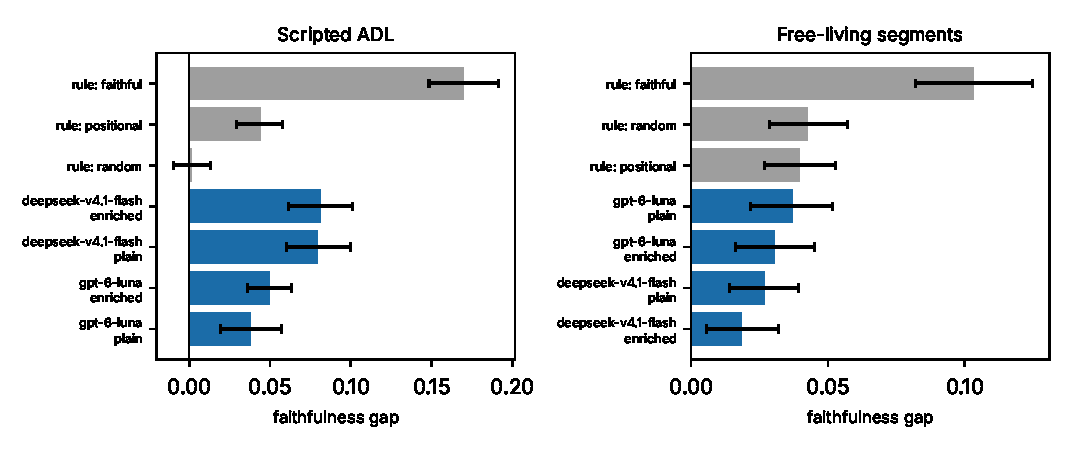
\includegraphics[width=\linewidth]{figures/explain_gap.pdf}
\caption{Faithfulness gap of each explainer with 95\% intervals (blue: language models; grey: rule-based references). Higher is more faithful to the classifier's decision.}
\label{fig:explain}
\end{figure}

On the scripted data the faithful rule has a gap of \XAFaithfulGap{} and precision 1.00 by construction, the random rule \XARandomGap{} and the positional rule \XAPositionalGap. The language models fall between: gaps of \XALunaPlGap{} (GPT-6-Luna, plain) to \XADeepEnrGap{} (DeepSeek, enriched), at most half of the faithful rule, and precision of \XALunaEnrPrec{} to \XADeepPlPrec{} against a chance level of 0.22 to 0.25 (Table~\ref{tab:explain}, Figure~\ref{fig:explain}). The cited events are therefore informative about the classifier's decision, more than random citation, but they are far from the events the classifier used. On the 600 free-living segments the gaps for the language models, \XHDeepPlGap{} to \XHLunaEnrGap, are about twice that of random citation (\XHRandomGap, interval \XHRandomGapLo{} to \XHRandomGapHi) but less than half of the faithful rule (\XHFaithfulGap). Precision is close to chance: \XHDeepEnrPrec{} for DeepSeek with context against a chance level of \XHDeepEnrChance, and \XHLunaEnrPrec{} for GPT-6-Luna with context against \XHLunaEnrChance. The positional rule is the most precise non-faithful explainer there (\XHPositionalPrec{} against \XHPositionalChance), because the events at the start of an episode are often characteristic of it. A first run on 120 segments had suggested that the language models were no better than random citation. With five times as many segments the gap is above random but small, so the first conclusion was too strong; the precision result did not change.

These numbers need a careful reading. They measure agreement with \emph{this classifier's} evidence. A language model that explains from its knowledge of the activity (``the stove sensor fired, so the resident was cooking'') may be right about the world and still cite different events from those a bag-of-events classifier relied on. For understanding the world that can be a virtue. For accountability it is the problem: an explanation attached to an alert is read as the reason the \emph{system} raised the alert, and when it describes a plausible reason that was not the actual one, nobody can use it to audit the decision. The practical consequence for explain-only designs is that evidence should come from the decision model, with the language model asked only to put it into words. The faithful rule's gap of \XAFaithfulGap{} against at most \XADeepEnrGap{} for the language models' own choice of evidence shows what is lost by letting the language model choose.

\section{From measured faithfulness to accountability}
\label{sec:accountability}

This section uses EU and Vietnamese law as a lens on the three questions an AAL deployment raises: what evidential weight a model-generated inference can carry, whether the monitored older adult has consented to it in a meaningful way, and who answers when it is wrong. It is an analysis for researchers and practitioners, not legal advice. The EU material rests on the texts of the instruments cited; the Vietnamese material rests on the titles and effective dates of the instruments and on secondary commentary, and it needs confirmation by local counsel before reliance, in particular because implementing decrees are still being issued.

\subsection{The evidentiary standard a model-generated inference can meet}
A caregiver or a clinician who acts on an agent's alert is treating the inference as evidence of a state of the world: a fall, a missed medication, a wandering episode. What makes that reasonable is a track record and an account of why this alert was raised. Accuracy statistics supply the first. The second is exactly what an unfaithful explanation destroys, and what a faithfulness score partially supports. An audit can ask: for this alert, did the evidence the agent cited actually drive the conclusion? If $F$ for the system is indistinguishable from zero, then the explanation attached to any single alert carries no information about why it was raised, and it should not be given probative weight in a dispute. If $F$ is clearly positive, the explanation is a better, though still imperfect, guide to what to look at.

Several legal provisions make explanation quality more than a courtesy. Under the GDPR a data subject is entitled to ``meaningful information about the logic involved'' in automated decision-making (Arts.~13(2)(f), 14(2)(g), 15(1)(h)), and the Court of Justice has held that this requires an explanation that allows the person to understand the procedure and principles applied, not the algorithm itself, and that the controller cannot hide behind trade secrets without the explanation being tested by the competent authority or court (Case C-203/22, \emph{Dun \& Bradstreet Austria}) \cite{cjeu_dnb}. An explanation that is fluent but unrelated to the decision cannot satisfy this. The AI Act adds, for high-risk systems, requirements on transparency to deployers (Art.~13), on accuracy and robustness (Art.~15), and a right of an affected person to a clear and meaningful explanation of the role of the system in a decision that has legal or similarly significant effects on health, safety or fundamental rights (Art.~86) \cite{aiact}. A measurement that shows whether the explanation tracks the decision is directly relevant evidence of compliance.

A further point concerns the status of an alert as a ``decision''. The Court of Justice held in Case C-634/21 (\emph{SCHUFA}) that producing a score is itself an automated decision under Art.~22 GDPR when a third party draws strongly on it \cite{cjeu_schufa}. By analogy, an AAL agent whose alerts a caregiver or a care provider habitually follows may be performing automated decision-making in the sense of Art.~22, even if a human formally ``decides''. Where the human in the loop only confirms, the oversight is nominal, and the faithfulness of the explanation is what makes confirmation more than a click.

\subsection{Consent and the monitored older adult}
AAL systems process health-related data about a person who is often frail and sometimes cognitively impaired. Under the GDPR this is special-category data (Art.~9(1)), and automated decisions based on it are restricted further (Art.~22(4)): they may rest only on explicit consent or substantial public interest, with suitable safeguards. A data protection impact assessment is required where processing is likely to result in high risk (Art.~35), which continuous monitoring of vulnerable people plainly is. Three features make consent difficult. Consent must be freely given, and recital~43 warns that it is not where there is a clear imbalance between the parties; an older adult whose place in a care home or whose family's willingness to let them live alone depends on accepting monitoring is not in a position of free choice. Consent must be specific and informed, and a person cannot be informed about reasoning that the system cannot faithfully report. And consent must be revocable, which in a shared home means that the choice of one resident should not expose the others.

The faithfulness protocol helps with the second point, concretely. A consent notice that promises ``you will be told why the system raised an alert'' is only truthful if the explanation is a reliable guide. A deployer who has measured $F$ can say what the explanation is: faithful to the degree that this score shows. A deployer who has not measured it is promising something it cannot know. Data minimisation (Art.~5(1)(c)) also points to sufficiency: if the cited events alone carry the conclusion, the system may not need to retain the rest.

In Vietnam, the Law on Personal Data Protection (Law No.~91/2025/QH15), in force from 1 January 2026, and the preceding Decree 13/2023/ND-CP distinguish basic from sensitive personal data, rely on consent as the primary legal basis, and require impact assessments; health information is within the sensitive category under the framework that preceded the Law \cite{vn_pdpl}. Vietnamese law on older persons recognises the rights and care of the elderly (Law on the Elderly, No.~39/2009/QH12) without addressing AI monitoring. The practical position is therefore close to the EU one: explicit and informed consent, an assessment before deployment, and special care where the person cannot readily refuse.

\subsection{Allocating responsibility}
In the EU, the AI Act distributes obligations by role. A system that dispatches or prioritises emergency first-response services, including medical aid, is listed as high-risk in Annex III (point 5(d)); an AAL monitor that is marketed for a medical purpose may in addition be a medical device under Regulation (EU) 2017/745 and so fall into the high-risk category through Art.~6(1). Providers must provide documentation, accuracy and robustness testing, and instructions for human oversight (Arts.~9, 13--15). Deployers must use the system according to the instructions, assign oversight to people with the necessary competence and authority, monitor operation, keep logs, and report serious incidents (Art.~26) \cite{aiact}. The oversight that Art.~14 requires includes being able to ``correctly interpret the output'' and to remain aware of automation bias, both of which depend on explanations that mean what they say. The date on which these obligations start to apply was postponed for stand-alone high-risk systems by the Digital Omnibus amendment, reported to take effect from 2 December 2027, with later dates for products under sectoral law; the dates should be checked against the Official Journal when planning a deployment \cite{omnibus}.

For compensation, the picture is changing. The revised Product Liability Directive (EU) 2024/2853 brings software, including AI systems, within the definition of a product and provides for strict liability for defects, disclosure of evidence and rebuttable presumptions of defectiveness in some cases, and Member States must transpose it by 9 December 2026 \cite{pld}. The proposed AI Liability Directive has been withdrawn. This matters for faithfulness. A claimant harmed by a missed fall will find it hard to show why a model failed, and a provider who has run a protocol like ours holds exactly the kind of evidence that disclosure rules may reach. Deployers and caregivers remain exposed under national tort and professional-negligence law, and there the key question is whether it was reasonable to rely on the system's output given what was known about its reliability.

In Vietnam, the Law on Artificial Intelligence (Law No.~134/2025/QH15), adopted in December 2025 and in force from 1 March 2026, adopts a risk-based approach with higher-risk systems subject to stronger obligations, and gives existing systems in sectors including health care a longer transition period (reported as 18 months, against 12 months for others); the detailed classification criteria and incident-reporting rules are being left to implementing decrees \cite{vn_ailaw}. Civil liability for harm outside a contract is governed by the Civil Code of 2015 (Arts.~584--585), whose general rule is liability for fault with an obligation to compensate in full. Whether the strict liability rule for sources of extreme danger (Art.~601) applies to software is doubtful and, to our knowledge, untested.

\subsection{An allocation by who controls which failure}
False alarms and missed events fall differently on the parties, and a useful allocation follows who can control each failure. \emph{Developers} control the model and its documentation: reported accuracy, calibration, and faithfulness as measured. A developer who ships an explanation feature without testing whether it is faithful is responsible for the consequences of presenting a possibly spurious account as reasoning. \emph{Deployers} (care providers, housing associations, operators) control the configuration, the thresholds, the escalation policy and the training of staff; they are responsible for deciding which actions the agent is allowed to take, which is the subject of the next section. \emph{Caregivers} control the moment of action: they decide whether to act on an alert. Their responsibility should be bounded by what they could reasonably know. A caregiver told that the explanation is an unverified narrative has been given an accurate picture; one who is shown the same text as a reason has not.

\section{A graduated authority ladder for agent actions}
\label{sec:ladder}

The ladder gives the measured evidence a decision role. It has four levels, ordered by the harm of a wrong action and by how hard it is to undo.

\begin{center}
\small
\begin{tabular}{@{}cp{4.4cm}p{6.4cm}@{}}
\toprule
Level & Permitted action & Conditions \\
\midrule
0 & Log only & Always allowed. Required if the answer rate is below 95\% or the noise floor exceeds 10\%. \\
1 & Notify a caregiver, showing the cited evidence; the explanation is labelled unverified & Lower accuracy bound $\ge 0.80$. \\
2 & Reversible automated action (prompt the resident, adjust lighting) & Lower accuracy bound $\ge 0.90$ and lower bound of $F$ above zero. \\
3 & \emph{Propose} an irreversible or high-harm action (emergency call, medication change) & Lower accuracy bound $\ge 0.95$ and lower bound of $F\ge 0.5\,F_{\mathrm{ref}}$. A human always confirms. \\
\bottomrule
\end{tabular}
\end{center}

Four design choices deserve comment. The conditions use lower confidence bounds, so that a small evaluation cannot buy authority. They are cumulative, so that no explanation score can compensate for poor accuracy and no accuracy can compensate for an explanation that does not track the evidence. The faithfulness threshold is relative to $F_{\mathrm{ref}}$, the score of a reference agent that is faithful by construction on the same data, because $F$ has no absolute scale (Section~\ref{sec:reference}). Level 3 grants the right to propose, never to execute: no value of any measured quantity unlocks autonomous irreversible action, which keeps a person in the loop where the law expects one (GDPR Art.~22(3), AI Act Art.~14). The thresholds are policy parameters, not findings, and a deployer should set them with the clinical consequences of each action in view. The code applies the ladder to any set of protocol results (\texttt{faithaal/ladder.py}).

Applied to the reference agents in Table~\ref{tab:ref}, with $F_{\mathrm{ref}}=\FFaith$, the ladder gives the following. All three agents have the same accuracy lower bound, 0.925, which clears the level-1 and level-2 accuracy conditions but not the 0.95 needed for level 3, so none may propose irreversible actions. The faithful and the positional agents both reach level 2, because the lower bounds of their $F$ intervals are above zero. The random agent is held at level 1 because its interval contains zero. The result is partly reassuring and partly a warning. It shows the ladder withholding authority from an agent whose explanations are unrelated to its decisions even though its accuracy is the same as the others'. It also shows that the level-2 condition, $F$ above zero, is too lax to separate the faithful agent from the positional one, whose score is small but positive. A stricter relative threshold at level 2 would separate them; we have not adopted one because choosing it after seeing these numbers would be tuning the policy to the example, and the thresholds are for each deployer to set. This is an illustration of the mechanism on a simple classifier in a scripted setting. It does not show that any agent is safe to deploy.

Applied to the language-model configurations in Table~\ref{tab:llm}, the ladder gives level \MaxLevel{} to every one. The highest accuracy lower bound is \AccMaxLo, below the 0.80 needed for level 1, so on these data none of the agents may do more than log. The faithfulness scores, whatever they show, would not change this: the ladder is cumulative, and accuracy gates every level above logging. This is the practical answer to the question in the title for this pilot. On scripted activities that a logistic regression recognises 95.8\% of the time, none of the language-model configurations tested is accurate enough to be allowed to notify a caregiver on the strength of its own reading.

\subsection{The ladder with the decision held fixed}
Table~\ref{tab:explain} also shows what the ladder does when the decision system is the same and only the explainer differs. On the scripted data the decision accuracy is the same for every row, \DecAccAdl\% with a lower bound of \DecAccAdlLo\%, which allows level 2 at most. Under the default policy (Level A) the random explainer is held at level 1 and every other explainer reaches level 2: the default policy separates explainers with no relation to the decision from the rest and nothing finer, as in Section~\ref{sec:ladder} above. Under a stricter alternative (Level B), which requires the lower bound of the faithfulness gap to be above zero at level 1 and at least a quarter of the reference value at level 2, the random explainer falls to level 0, the positional explainer and the GPT-6-Luna explainers to level 1, and the faithful rule and the DeepSeek explainers stay at level 2. The same decisions, at the same accuracy, are thus allowed different authority depending only on how well the explanation tracks them. We defined the alternative policy after seeing the gaps of the first scripted experiment, so it is a sensitivity analysis and not a validated threshold. On the free-living segments the decision accuracy lower bound is 0.56 and every explainer sits at level 0 under both policies: the ladder is cumulative, and no explanation quality compensates for an unreliable decision.

\subsection{What the pilot says about the question}
Taken together, the experiments give a more specific answer than ``do not trust language models''. (i) Recognition quality depends strongly on whether the sensor data carry meaning: weak with opaque identifiers, on par with a trained classifier with meaningful names. (ii) Neither accuracy nor a fluent explanation tells you whether the explanation reflects the decision, and the two are only loosely related. (iii) Where the decision is made by a model whose evidence is known, language-model explanations track that evidence only modestly better than chance on scripted data and barely above chance on free-living data, which is a measurable gap and a design choice, not a law of nature: take the evidence from the decision model. (iv) The authority an agent may hold can be tied to these measurements in steps, so that the same system is allowed to log, to notify, or to propose, depending on evidence about the decision and about the explanation separately, and so that irreversible actions always keep a human in the loop.

\section{Limitations and open research directions}
\label{sec:limits}

\paragraph{Sensitivity is necessary, not sufficient.} A positive $F$ shows that the cited events matter to the conclusion. It does not show that the conclusion is right for the right reasons: an agent may cite the correct sensor and use it through a spurious rule. Faithfulness to a wrong mechanism is still faithfulness. A high $F$ should lower our worry about confabulation and leave our worry about unsound reasoning where it was.

\paragraph{Redundancy limits power.} When the evidence is redundant, removing the cited events does not change the answer even if the explanation is faithful, so $F$ understates faithfulness for such agents. Calibrating against a reference agent mitigates this but does not remove it. Finer measures, such as changes in label probabilities, are unavailable for models that expose only text.

\paragraph{Intervention realism.} Interventions can produce logs that never occur in a home. Inverting a reading or deleting an event may yield physically impossible sequences, and an agent may then change its answer for the right reason: because the log has become incoherent. The matched control reduces this confound but cannot eliminate it. Interventions that preserve plausibility, for example by sampling replacements from a model of the home, are an open direction.

\paragraph{Scope of the pilot.} The data are scripted, short, single-resident and recorded in one apartment. Free-living data are longer, noisier and involve visitors and pets, which affects both accuracy and the meaning of an intervention. The reference agents are not language models, and the validity check shows that the protocol can tell citing rules apart, not how language models behave. The language-model study is small and uneven. Only two models were run on all recordings. Three others were run on 15 or 20 recordings and, for three of them, the plain prompt only. Each configuration was run once at temperature zero, so run-to-run variation beyond the null control is not measured. Prompts were written once and not tuned, models were served through third-party aggregators whose versions can change, and optional reasoning modes were switched off, which may lower accuracy. Several attempted configurations produced too few answers to report and are excluded: Ministral-8B (Mistral API) and the free MiniMax-M3.1-Flash and Nemotron-3-Ultra models returned answers for fewer than 15 recordings because of rate limits, the Gemini model was unavailable because of persistent overload, and the enriched-prompt runs for the three Groq models stalled on daily token limits. The raw records of the excluded Mistral run are kept in the repository. The two later experiments add their own limits. The free-living task classifies episodes whose boundaries are given, which is easier than the real problem of finding them in a continuous stream; it uses 600 sampled episodes (240 for the full protocol, plain prompt only), eight merged activity classes and logs of at most 80 events. The explain-only experiment measures agreement with one bag-of-events classifier, which is a stand-in for a decision model, and says nothing about explanations of a model whose evidence is less transparent. The free Laguna model was excluded from both new experiments because it stalled on rate limits. The protocol and code, not the particular numbers, are the contribution of this section.

\paragraph{Legal scope.} The legal analysis is a research synthesis. Regulations are moving: dates under the AI Act have recently shifted, the Vietnamese implementing decrees are incomplete, and case law on explanation duties is young. Vietnamese material needs verification by local counsel. The ladder's thresholds are policy choices that must be made for each deployment.

\paragraph{Open directions.} We see four: testing faithfulness under realistic, plausibility-preserving interventions; extending the protocol from single-recording classification to day-long streams where an agent acts on partial evidence; studying how caregivers actually use explanations, since the benefit of faithfulness depends on human behaviour that we have not measured; and establishing, with clinicians and regulators, which thresholds are acceptable for which actions.

\bibliographystyle{plainnat}
\bibliography{refs}

\end{document}
